
\chapter{Description du Travail}

La majorité de la littérature traite le problème de la reconnaissance d'après une seule image de l'objet. Typiquement, une ensemble de \textit{features} est extrait et, ensuite, comparé aux modèles d'objets présents dans une base de données initiale, en contraste aux méthodes directes, comme deep learning, où l'image d'entré est associée directement avec des classes des objets correspondants au compromis d'une étape d'entrainement importante, pour l'apprentissage de \textit {features}, encore plus dans un espace à 3 dimensions provenant du capteur RGB-D. 

Un grand effort était fait pour améliorer l'extraction, le \textit {matching}, ainsi que le \textit{features} elles-mêmes pour qu'elles soient invariantes à transformations affinés de l'image et représentatives de l'objet. Ce traitement classique a l’avantage d'être, à la fois modulaire, avec des étapes bien définies de segmentation, Extraction de features, classification et post-traitement, et, au même temps, d'avoir des résultats satisfaisants d’après une implémentation plus immédiate. Malgré son intérêt dans certains cas, rapidement on s’aperçoit de limitations lors que vues ambiguës apparaissent.

L'utilisation d'un algorithme de reconnaissance basée sur une seule image apporte l'inconvénient de
n'incorporer pas les notions de vue et de transition entre elles, au contraire, la majorité de ces systèmes souhaitent être invariant à les
vues d'objets, en autres mots, avoir la capacité de l'identifier de n'importe quel point de vue. Un système dérivé de celui-ci pourrait
traiter le concept de vues plus représentatives et transitions, par contre, de façon moins intuitive. De cette manière, les articles présentés
auparavant travaillent sur le domaine multi vue, incorporant des aspectes géométriques, pour augmenter la qualité de son estimation.

En dernière analyse, l'objectif ultime c'est d'avoir une reconnaissance multi vue, en
instance, capable d'incorporer son déplacement pour résoudre des
ambiguïtés et faux positifs. Pour incorporer les notions voulus, on présente, simultanément,
un simple modèle d’objet suffisamment général et un système capable
d'estimer l'orientation de l'objet reconnu, ou bien un système de
reconnaissance de vue, pour, ensuite traiter l’information motrice du
robot pour augmenter le taux de réussite.

\section{Segmentation}

La segmentation consiste de la soustraction des objets d'une image brute, en autres mots, différencier les éléments non constituent du
objet de lui-même. La compréhension de la continuité des objets est
considérée comme un défi majeur dans le traitement d'image étant
donné qu'une fois l'objet séparé du fond, la reconnaisse devient
beaucoup plus évident. Une énorme partie de sa difficulté vient du fait
de la projection de la scène dans le plan supprimer l'information
correspondant à distance. Les capteurs stéréoscopiques et
infra-rouges ont recomposé cette absence d'information et simplifié
énormément le traitement nécessaire pour obtenir des objets
potentiels. Les cartes de profondeur pourraient être utilisées pour
représenter cette nouvelle information, pourtant, encore plus
naturelle, le concept de nuage de points propose une représentation
spatial en trois dimensions de l'environnement capturé.

La démarche proposée par la littérature considère les objets comme des
ensembles de points définis par un seuil initial de proximité. Cette
définition est bien extensive et permet de représenter une énormité,
sinon tous, les objets. Néanmoins, définir ces ensembles dans une
image brute n'est pas tout à fait simple. En conséquence, un nouveau à
priori qui spécifie que les objets se placent sur des plans de
support, malgré plus restrictif que la définition d'avant, permet un
segmentation crédible.

\subsection{Algorithme}

La méthode de segmentation de l’algorithme Tabletop
se base exactement sur ces aprioris. Pour retrouver les objets posés
sur une table, l'algorithme recherche récursivement les plans de
support, où le plus important est pris comme la table. Autrement,
l'article {\color{blue}ENSTA}, en partant du même principe, propose un
traitement pour le fond de la scène, où les plans orthogonaux à
normale du sol et de taille suffisamment grand sont considérés comme
des murs, orientés à segmentation d'objets dans les environnements
intérieurs. Ainsi, la dernière segmentation, proposé par *Luis
Charles*, répond aux exigences du domaine de déplacement du robot: le
laboratoire de Thales, Theresis.

Plus spécifiquement, elle peut être découpée dans les étapes suivantes
:

\begin{enumerate}
\item Soustraction du sol... {\color{blue} DETAILLER}

\item Filtrage de points distants, considérés comme plus incertains.

\item Calcul de la normale des superficies comprises dans la scène

\item Élimination de murs, considérés comme de plans orthogonaux au
sol de taille suffisamment grande, d'après un seuil.

\item Projection des points appartenant aux objets dans le plan du
sol.

\item Détermination de l’enveloppe convexe correspondant au sol détecté.

\item Réduction de la densité de discrétisation pour accélérer l'étape
de \textit{clustering}.

\item Clustering des objets par l'algorithme *point growing*

\item Retour à discrétisation initiale.

\item Calcul du centroïde et \textit{bouding boxes} 2D et 3D

\item extraction d’imagettes, et autre informations pertinents aux
objets détectés.
\end{enumerate}

Une calibration initiale est nécessaire pour définir l'équation du
sol. Pour cela, on place le robot dans un endroit de façon que l'image
aperçue correspond majoritairement au sol. L’équation du plan plus
important, plus grand nombre de points dans le nuage, est extrait par
le RANSAC et sauvegardé dans un fichier texte. Une explication plus
détaillée sur les sous-méthodes utilisées pour chaque étape, telle
comme le RANSAC est présentée dans les annexes, ainsi comme une
discussion des paramètres utilisés.

\subsection{Restrictions} Les physiques de capteurs restreins les
types d'objet qui peuvent être aperçus et, ensuite, segmentés, soit à
cause de l'interaction avec les rayons infra-rouges, soit à cause de
résolution limitée des images mesurées. Dans l'autre côté, la
segmentation a ses propres contraints concernant le positionnement des
objets dans l'image et, principalement, la définition de sol et murs,
résultant dans les restrictions suivantes :

\begin{itemize}

\item L'objet se trouve par terre.

\item L'objet se trouve au centre de l'image
\item Ambiant isolés de lumière infra-rouge 

\item Le sol où le robot se déplace n'est pas accidenté.


\item L'objet se trouve à une distance inférieure à 3 mètres 


\item L'objet est assez grand et dépasse le seuil d'appartenance au
sol.

\item L'objet n'est ni transparents et ni trop réflective.

\end{itemize}

Un grand nombre d'objets, entre chaises tables, écrans, boîtes en
carton, poubelles, de tailles et formes variés étaient testés et
peuvent être segmentés malgré les restrictions listées. Quelques
exemples de segmentation sont présentés dans les annexes pour illustrer
la capacité de segmentation.

\section{Descripteurs}

Le travail des descripteurs est, d'un côté, de comprendre les
caractéristiques intéressants et, d'un autre, de réduire la
dimensionnalité du espace traité, tandis que restant robuste à des
transformations affines et changement de luminosité. On classifie les
descripteurs selon la caractéristique qu'il exprime. Une première
group sont les descripteurs géométriques qui essaient de traduire les
idées de courbure, forme et taille dans histogrammes, et sont intéressant
 pour etudier les ambiguïtés de reconnaissance, un fois que la plus parts 
 d'objet ont une certaine symétrie spatiel.

\subsection{Point Feature Histogram - PFH}

Le PFH incorporé les notions de courbure des objets par le calcul de
l'écart entre les normales de points. Ce descripteur peut être calculé
localement ou globalement, en changeant l'importance du rayon de
comparaison. Il est la base d'une grande famille de descripteurs, desquels
quelques-uns seront expliqués dans la suite.

En revenant à son calcul, l'histogramme est évalué à partir des pairs
de points à l'intérieur d’un ensemble prédéfini. D'abord, un repère
initial, illustré dans l'image *9* est établis sachant le vecteur distance normalisé et les deux
normales. Ensuite, trois angles, qui correspondent à la transformation
angulaire entre les deux normales, et la distance euclidienne entre le
deux points sont estimés. Ces quatres valeurs seront considérés comme
features pour réduire l’espace initial de douze dimensions - coordonnées
et normales des dois point - à un espace de quatre dimension.


\begin{equation*}
  {\mathsf u} = \boldsymbol{n}_s \qquad
  {\mathsf v} =  {\mathsf u} \times \frac{(\boldsymbol{p}_t-\boldsymbol{p}_s)}{{\|\boldsymbol{p}_t-\boldsymbol{p}_s\|}_{2}}  \qquad
 {\mathsf w} = {\mathsf u} \times {\mathsf v}
\end{equation*}

\begin{figure}[H]
\centering
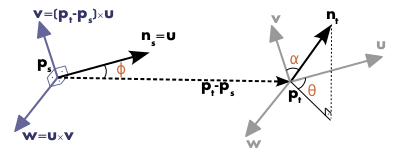
\includegraphics[width=0.6\textwidth]{pfh_frame.png}
%\caption{{\color{blue} Image d'explication du repère}.}
\end{figure}


Puis, les normales sont traduites en features angulaires décrit par les équations :
\begin{equation*}
  \alpha = {\mathsf v} \cdot \boldsymbol{n}_t  \qquad
  \phi   = {\mathsf u} \cdot \frac{(\boldsymbol{p}_t - \boldsymbol{p}_s)}{d} \qquad
  \theta = \arctan ({\mathsf w} \cdot \boldsymbol{n}_t, {\mathsf u} \cdot \boldsymbol{n}_t) \qquad
  d={\|\boldsymbol{p}_t-\boldsymbol{p}_s\|}_2 
\end{equation*}

La prochaine étape c'est de calculer l'histogramme en-soi. Un
subdivision du range de valeur de chaque feature angulaire, 
normalisés pour rester dans le même intervalle trigonométrique,
est faite et chaque cellule du histogramme est incrémenté dès
qu'une feature tombe dans cet intervalle. 

Le PFH se présente robuste à des différents échelles de densité de points et de bruit, au même temps que invariant à les transformations affines. Des inconvénients vient de la dépendance de la qualité de l'estimation de la normale\footnote{ Une discussion des méthodes présentés sur PCL est mis dans les annexes.}.

\subsection{Fast Point Feature Histogram - FPFH}

L'avènement du FPFH viens de la motivation de réduire la complexité de
calcule du descripteur PFH, $ O(nk^2) $, pour un nuage avec $n$ points 
où chaqu'un des points à $k$ voisins . Pour cela, l'algorithme au
lieu de calculer la relation bidirectionnelle entre tous deux points 
de l’ensemble définis, les features de chaque point sont pondérées 
par les voisins à l'intérieur d'un rayon de recherche, selon la formule
au-dessous :

$$FPFH(\boldsymbol{p}_q) = SPFH(\boldsymbol{p}_q) + {1 \over k}
\sum_{i=1}^k {{1 \over \omega_k} \cdot SPFH(\boldsymbol{p}_k)}$$

Cette procédure résulte dans une complexité O(n*k). Le gain en vitesse est considérable,
ce qui permet des applications en temps réelles. De plus, pour éviter une perte d'information considérable, le FPFH
incorpore quelques point externes au rayon de voisinage, mais que sont compris dans un rayon de taille.

\subsection{Viewpoint Feature Histogram- VFH}

Le VFH, différemment du rapport entre PFH et FPFH, c'est une extension
du deuxième descripteur où la variance de point de vue est prise en
compte. De forme succincte, des angles entre la normale de chaque point
et la direction principale d'observation est concaténée à l’histogramme
provenant du SPFH (Simplified PFH). En gardant le repère utilisé dans
les descripteurs d'avant, le vecteur direction principale est défini
par la différence entre l'origine du capteur jusqu'au centroide du
\textit{cluster}. Ce résultat permet, au même temps, de reconnaitre
l'objet et son orientation spatiale, et, par conséquent, c'est le
feature utilisé dans les premières expériences.

\subsection{Clustered Viewpoint Feature Histogram - CVFH} CVFH -
Clustered VFH - est une feature semi-global capable de gérer
occlusions partiels, mauvaise segmentation et bruit par la
décomposition du \textit{cluster}, segmenté comme objet, en sous-clusters de
structure spatiale homogène. Le descripteur est obtenu d'après un premier
filtrage de zones de haute gradient de courbure, considérés comme zones de
transitions entre surfaces, et, puis, et l'estimation de l'histogramme VFH pour chaque surface 
donnée par l'algorithme \textit{point growing}. Ainsi, pour un seul objet, le CVFH ne
généré pas un seul histogramme VFH, mais un vecteur des histogrammes.
En revanche, le découpement exige un soin un plus avec la résolution des surfaces pour
quelles restent représentatives de l'objet.

\begin{figure}[H]
	\subfloat[PFH ]{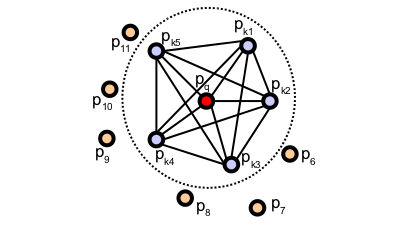
\includegraphics[width=4.5cm]{pfh_diagram.png}}
	\subfloat[FPFH]{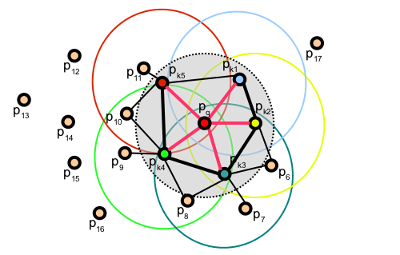
\includegraphics[width=4.5cm]{fpfh_diagram.png}}
	\subfloat[subcaption]{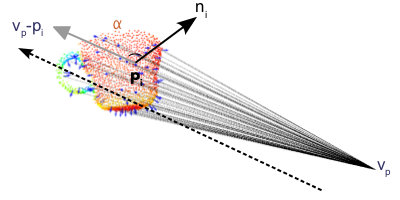
\includegraphics[width=6cm]{second_component.jpg}}		
\end{figure}

\section {Classification} L'étape de classification correspond à la différentiation entre les
histogrammes caractéristiques de chaque vue de chaque objet. Cette
mesure pourrait être apprise, par exemple, avec un réseau de neurone
ou n'importe quel autre méthode classique de \textit{machine learning}.{\color{green}Le travail * three dimensional
dof cluster vfh...* suggère l'utilisation de la mesure chi-squared
similarité entre histogrammes accouplé au classificateur k plus
proches voisins. }  Le grand avantage de ce classificateur c'est l'étape
d’apprentissage correspond à création d’un arbre de recherche,
construit d'après la comparaison croisée entre les éléments de la base,
que pour l'ordre de grandeur de la base de données envisagé, est
presque instantané.

L'API de la librairie FLANN sur PCL permet l'utilisation directe du classificateur
K - plus proches voisins. L'implémentation permets l'utilisation de plusieurs
définitions de distance entre histogrammes. La définition par défaut, Chi-squared,
dont la formule est décrit dans la suite, semble être capable de bien différentier
les histogrammes d'entrés, $H_1$ et $H_2$, et était choisi comme la définition pour le classificateur.

$$\sum _I \frac{\left(H_1(I)-H_2(I)\right)^2}{H_1(I)} $$


% Une étude des mesures de corrélation entre histogrammes peut être
% intéressant. Ces mesures sont classifié en deux classes : croisés et
% directs. La comparaison direct prend en compté différences par rapport
% à la même cellule de l’histogramme. Pendent que la comparaison croisée
% permet la comparaison entre cellules, par une matrice de
% corrélation. Les features géométriques ont des cellules bien définis
% et statiques, ainsi, semble plus naturel d'utiliser une comparaison
% \textit{bin-to-bin}.

% *Formula do site*

% \subsection{bin-to-bin} Comparaison entres cellules équivalents

% \begin{itemize}
% \item Correlation :
% \item Intersection :
% \item Bhattacharyya distance :
% \end{itemize}

\section{Représentation de l'objet}

Ces choix débouchent sur un système fonctionnel de reconnaissance de
vue qui permet de s’intéresser, ensuite, par le couplage de résultat de la
reconnaissance avec les informations de déplacement du robot.

{\color {green}
\subsection {Principes de la Reconnaissance Humaine}

Commençant par le modèle de l'objet, le but c'est de intégrer et
respecter certains principes appris après observation dans la
reconnaissance chez les humains :

\begin{enumerate}
\item Gazltat : Tendance à retrouver des formes et contours simples et
naturels par regroupement de caractéristiques et/ou comportements.

\item Continuité : l'apprentissage d'un nouvel objet se fait de forme
continue. Dans le cas discret, cela revient à un modèle qui simule les
transitions entre superficies.

\item Temporalité et séquentialité : Des études {\color{blue} ref} suggèrent que l'ordre
de visualisation de surfaces des objets influence sa reconnaissance à
posteriori. Par conséquent, la séquence spatiale entre vues joue un rôle sur le concept d'objet, où parcourir
séquence dans la même ordre que celle appris apporterais plus d'information.

\end{enumerate}

Malheureusement, avoir tous ces principes est une tâche assez complexe
pour l’état courant de la technologie, pourtant, en même temps, ils inspirent
possibles solutions et représentations. L'apport de cet étude se place dans les
domaines de la temporalité et séquentialité.

\subsection{Caractéristique des objets} 

En regardant dans la perspective des objets, certaines de ses caractéristiques sont utiles pour le différencier un des autres:

\begin {enumerate}
\item Taille
\item Position global
\item couleur et texture
\item Contraintes d’espace
\item Contexte dans l'environnement
\item Forme géométrique : 
\subitem Sous formes primaire 
\subitem Position et orientation relatif entre formes primaires
\item Affordance : se réfère au concept d’interactions possibles
avec un objet. De manière illustratif, dans le cadre du robot utilisé,
cela reviendrait à capacité de pousser un certain objet, d’où
l’intérêt de l’identification de l’orientation de l’objet.
\end{enumerate} 
}

Le modèle proposé doit être capable d'exprimer au
mieux ses caractéristiques en restant, encore, simple.  En reprenant la
discussion de l'état de l'art, on présent quelques modèles usuellement
utilisés pour représenter les objets en trois dimensions.

\subsubsection{Modèle CAD}

Consiste à représenter l'objet par son modèle 3D fait à l'aide d
outils de design numériques. L'avantage vient du fait d'une fois le
modèle construit, la visualisation de l'objet de n'importe quel vue
devient évident. De l'autre côté, la fiabilité du modèle est
intérieurement lié à la précision de la reconstruction 3D de l'objet,
où un soin avec l'échelle et dimensions, ainsi que avec la
reproduction de la couleur et texture, est important pour la bonne
représentativité.

\subsubsection{Évolution de contours}

Une autre approche est basé sur les silluettes des objets et leur
évolution d'après transformation affines. Cette problématique c'est
démontre mathématiquement compliqué au niveau de la modélisation de
fonctions de contour et de leur transformation. Cependant, une fois
modélise, une prévision

\subsubsection{Squelettes}
...

\subsubsection{Aspect-Graphs}

Cette forme de représenter les objets consiste à avoir un graphe où
chaque nœud correspond à une image d'un point de vue et les liens
entre nœuds les réelles transitions visuelles. Comme avoir un graphe
complet, qui s'approche du continue, apporte une besoin mémoire
important et une certaine redondance d'information, la préoccupation
principale est de trouver des point de vues représentatives, nommés
\textit{key-Frames}, qui peuvent être choisi avec politiques suivants:
\begin{enumerate}
\item Aléatoire : Ces key-frames peuvent être choisies de forme
complètement aléatoire. Absence de calcul intermédiaire ou
prétraitement.

\item Intervalle constant : Une façon simple c'est de conditionner les
\textit{key-frames} à un écart angulaire fixe. Cela permet d'unifier
le nombre de frames pour chaque objet, ce qui peut être intéressant
pour certaines applications

\item Événement visuels : Cela correspond à déterminer des grands
variations d'intensité des features pour estimer les key-frames plus
représentatifs de l'objet. L'inconvénient vient du besoin d'un
prétraitement, en plus, orienté différemment pour chaque feature,
lors de la création de la base de données.

\end{enumerate}

\section {Graphe d'aspect polaire}

On considère que les objets sont décrits par deux dimensions
d'information : une spatiale, concernant la position absolu de l'objet
dans l'environnement et les positions relatifs où l'objet était
visualisé, et une autre visuelle, donnée par les descripteurs
géométriques, de couleurs et de texture; qu'on cherche à transporter
dans un référentiel unique. Le graphe d'aspect permet de coupler
l'ensemble d'images suivant ses possibles transitions spatiales ce qui
résulte dans la possibilité de construire le modèle à la volée et de
jouer avec sa densité d'information - nombre d'images incorporées.

\begin{figure}[H]
\centering
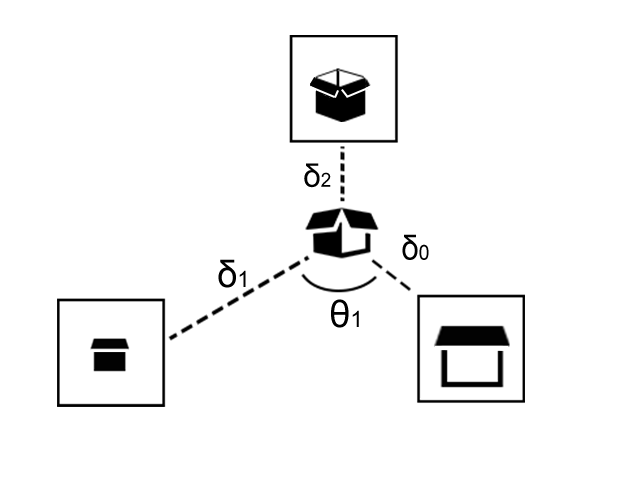
\includegraphics[width=0.4\textwidth]{object_model.png}
\caption{Fonction \`{a} \^{e}tre optimis\'{e} et la solution voulu.}
\end{figure}

Formellement, un référentiel polaire entrelace toutes ces informations
de façon à représenter la position spatiale d'où l'observation était
fait, tel comme il est représenté dans l'image *7*. Pour la
construction du modèle les conventions suivantes étaient adoptées :
\begin{itemize}
\item l'angle zéro est attribué à la première observation
\item L'origine du référentiel est la position globale de l’objet
\item Les features sont labellisées d'après le déplacement angulaire
et la distance au centroïde de l'objet.
\end{itemize}

Une grande majorité de features visuelles sont variantes à échelle, une
fois que la résolution de l’image joue un rôle assez critique pour la
détection de features, comme les patches SIFTs. Ainsi, avoir la distance
que l’image étais prise peut être intéressant pour limiter la
classification à une échelle valable.

\section{Filtre de Kalman }

La modélisation des objets entraîne le besoin initiale de les
localiser dans la scène pour, postérieurement, les identifier. À cause
de la divergence de l'odométrie, la mauvaise segmentation et le calcul
du centroïde de l'objet, la position estimée est fortement bruitée
ayant un écart type qui rend la suive et identification infaisable
lorsque plusieurs objets sont minimalement proches. Un filtre de
Kalman ayant un modèle unitaire pour la matrice de transition d'états,
moyenne les observations pour s'adapter au bruit de mesure.

Cependant, le caractère monomodal du filtre de Kalman fait en sorte
qu'un seul objet cible peut être suivis à la fois. Pour atteindre
l'aspect multimodal, il faut que plusieurs filtres tournent en
parallèle. Ainsi, le problème passe d’estimer la position à décider
quelle observation appartient à quel filtre, l'étape
d'identification. Cela se fait à l'aide d'une matrice de corrélation
de distances entre les nouvelles observations et les états courants de
chaque filtre existant. Une solution simplificatrice est d'associer
chaque observation au filtre selon l'ordre de vraisemblance de cette
matrice. Lorsqu’une ambiguïté se produit dans l'étape
d'identification, la classification peut aider à prendre une décision
de mettre un filtre à jour ou, alors, créer un nouveau filtre.

\section {Chaînes de Markov Cachées}

Le déplacement physique du robot résulte dans une séquence
d'observations, en angles différents, d'un même objet. On exploit
l'information odométrique entre les visualisations pour prédire les
prochaines possibles orientations. De cette manière, l'évolution de la
reconnaissance au long du temps est représenté par un processus
stochastique, dont une modélisation possible correspond à le traiter
de façon discrète dans un espace d'état. Ayant l'apriori que la
dernière image et le dernier déplacement suffisent pour faire cette
prédiction, en respectant, donc, la propriété de Markov de premier
ordre, le processus stochastique est modélisée sur le cadre d'une
chaîne de Markov cachée.

Concrètement, les états cachées correspondent à des objets connus au
préalable et déjà incorporés dans la mémoire du robot. Cela contraint le
nombre d'états et on se rencontre avec un chaîne fini. Puis, une
matrice de transition décrit l'évolution du processus et c'est là où
l'odométrie et la relation entre vues et entre objets sont
incorporés. Finalement, une autre matrice, dit matrice d'émission,
estime la vraisemblance entre l'observation et les états de la
chaînes.

Une autre deuxième modélisation serait d'avoir une chaîne de Markov
Cachée distincte pour chaque objet et ensuite décider quel était le
processus le plus vraisemblable. Ce cas est un sous-ensemble du cas
antérieur où les transitions entre deux objets ne sont pas
considérés. Pourtant, ce qui peut être utile s'on considère
l'évolution d'objets, par exemple, la transition entre une chaise vide
et une personne assise sur une chaise ou encore un personne
commence à marcher.

\section{Déplacement du robot}

Le robot est équipé de trois roues, desquelles les symétriques
arrières sont motorisés et responsables pour le déplacement
motrice. Au même temps que la dernière sert à donner un support pour
la partie derrière du châssis. Les moteurs sont contrôlés à
partir de commandes sériel, préétablis pour le fabricant, qui
définissent la vitesse de roulement. La combinaison des rotations
des deux roues motorises dans les deux sens possibles permets au
robot d'avoir les comportements suivants:

\begin {itemize}
\item Déplacement en ligne droite : équivalent aux deux roues roulant
avec la même vitesse et dans le même sens.

\item Déplacement en arc de cercle : La différence entre les vitesses
de roues résulta dans un mouvement de cercle. Le rapport entre cette
différence permettre définir la courbature de la trajectoire.

\item Rotation : Dans ce cas, les deux roues sont commandées à la même
vitesse, mais avec de sens différents.
\end{itemize}

*Illustration*

Finalement, la combinaison de ces mouvements permet au robot de
accéder n'importe quelle position de l’espace.

\subsection{Estimation de l'odométrie}

Certains robots sont dotés de capteurs aptes d'estimer de façon
approximé sont déplacement. C'est aussi le cas du robot ciblé qui
possède encodeurs capables d'estimer la rotation angulaire des
roues. Une intégration, au sens mathématique, de la différence entre
l'odométrie entre deux intervalles de temps permet de retrouver la
position global du robot.

\subsection{Problèmes de déplacement}

La roulette de support originalement installée avait deux axes de
rotation. Pourtant, quelques mouvements de rotation du robot alignent
la roulette orthogonalement au sens du prochain mouvement ce qui crées
une torche parasite que perturbe la trajectoire voulue. Une tentative
frustrée d'installer une bille omnidirectionnelle à roulement, qui se
bloquait sur la moquette avec le poids du robot, a fait que
l'originale était réinstallée. Une deuxième solution serait d'interdire
certains mouvements du robot pour éviter cette déviation.

\subsection{Fusion de données}

L'estimation de l’odométrie diverge au long du temps dû à
l'accumulation d'erreurs mesure. Cette divergence est encore plus
considérable . Dans l'autre côté, l'utilisation du senseur RGB-D
estime la distance au centroïde de chaque objet. Une correspondance
entre les objets de deux observations consécutives nous donné une
autre repère de positionnement. Un couplage des deux mesure, une
provenant de l’encodeur moteur et l'autre du capteur infrarouge, fait
que l'odométrie doive être

\section{Architecture}

Le design de l'architecture sert à décider comment définir les unités de traitement et la communication entre elles. La définition des unités de traitement suit le découpage du pipeline de reconnaissance avec des nœuds responsables pour la segmentation, calcul de features et la classification, aussi comme, le contrôle du robot.

L'interfaçage matériaux-logiciel était fait sur l'environnement ROS -
Robot Operating System. Aussi que les outils d'affichage, ROS, 
rassemble les librairies d'acquisition d'images RGB-D, OpenNi 2 et Freenect, et de traitement de nuage de point, PCL.
De même, sa structure de nœuds a permis une implémentation modulaire et direct du
système décrit au-dessus, bien comme la communication entre machines, l'ordinateur portable et celui embarqué au robot.

L'image *10* illustre l'architecture en soulignant le flux d'information à travers des nœuds.




